\documentclass[twoside,10pt]{article}
\usepackage{amsmath,amsfonts,amsthm,fullpage,amssymb}
%\usepackage{mymath}
\usepackage{algorithm,amsmath,amssymb}
\usepackage{algorithmic}
\usepackage{graphicx}
\usepackage{url}


\begin{document}


\title{ISYE 6740 Homework 5\\ 
Fall 2020\\
\small Total 100 points + 10 bonus points.}
%\author{Yao Xie}
%\date{Deadline: Feb. 13, Sat., 11:55pm}
\date{}
\maketitle



%As usual, please submit a report with sufficient explanation of your answers to each the questions, together with your code, in a zip folder.

%----------------------------------------------------------------------------------



\begin{enumerate}


\item{\bf SVM. } (45 points)

\begin{enumerate}
\item (5 points) Explain why can we set the margin $c = 1$ to derive the SVM formulation?
\item (10 points) Using Lagrangian dual formulation, show that the weight vector can be represented as
\[
w = \sum_{i=1}^n \alpha_i y_i x_i.
\]
where $\alpha_i \geq 0$ are the dual variables. What does this imply in terms of how to relate data to $w$?
\item (10 points) Explain why only the data points on the ``margin'' will contribute to the sum above, i.e., playing a role in defining $w$. 

\item (20 points) Suppose we only have four training examples in two dimensions as shown in Fig. The positive samples at $x_1 = (0, 0)$, $x_2 = (2, 2)$ and negative samples at $x_3 = (h, 1)$ and $x_4 = (0, 3)$. 
%
\begin{center}
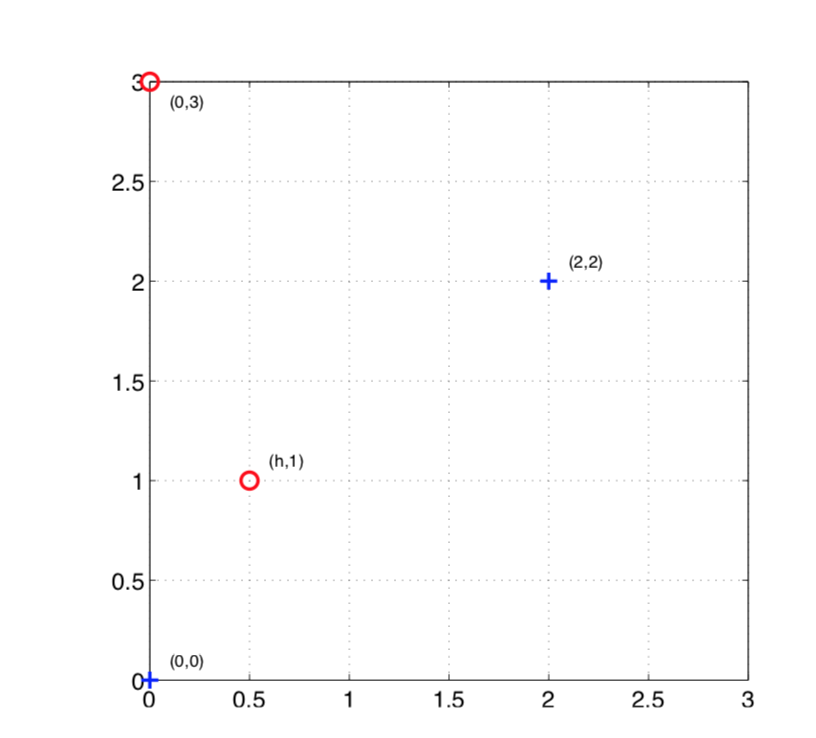
\includegraphics[width = 0.5\textwidth]{svm}
\end{center}

\begin{enumerate}
\item (10 points) For what range of parameter $h > 0$, the training points are still linearly separable?



\item (10 points) Does the orientation of the maximum margin decision boundary change as $h$ changes, when the points are separable?
\end{enumerate}
\end{enumerate}



\item {\bf Multi-class classification for MNIST data set, comparison.} (55 points)

This question is to compare different classifiers and their performance for multi-class classifications on the complete MNIST dataset at \url{http://yann.lecun.com/exdb/mnist/}. You can find the data file \textsf{mnist\_10digits.mat} in the homework folder. The MNIST database of handwritten digits has a training set of 60,000 examples, and a test set of 10,000 examples. We will compare {\bf KNN, logistic regression, SVM, kernel SVM, and  neural networks}. We suggest to use \textsf{Scikit-learn}, which is a commonly-used and powerful \textsf{Python} library with various machine learning tools. But you can also use other similar libraries in other programming languages of your choice to perform the tasks. Below are some tips. 

\begin{itemize}

\item We suggest you to ``standardize'' the features before training the classifiers, by dividing the values of the features by 255 (thus map the range of the features from [0, 255] to [0, 1]).

\item You may adjust the number of neighbors $K$ used in KNN to have a reasonable result (you may use cross validation but it is not required; any reasonable tuning to get good result is acceptable).

\item You may use a neural networks function \textsf{sklearn.neural\_network} with \textsf{hidden\_layer\_sizes = (20, 10)}. 

%Tune the step size so you have reasonable results. You may use \textsf{svc} and tune the penalty term $C$ to get reasonable results. 

\item For kernel SVM, you may use  radial basis function kernel, and a heuristic called ``median trick'': choose the parameter of the kernel $K(x, x') = \exp\{-\|x-x'\|^2/(2\sigma^2)\}$. Choose the bandwidth as $\sigma=\sqrt{M/2}$ where $M =$ the median of $\{\|x^i-x^j\|^2, 1\leq i, j \leq m', i\neq j \}$ for pairs of training samples. Here you can randomly choose $m'=1000$ samples from training data to use for the ``median trick''\footnote{Garreau, Damien, Wittawat Jitkrittum, and Motonobu Kanagawa. "Large sample analysis of the median heuristic." arXiv preprint arXiv:1707.07269 (2017).}.

\item For KNN and SVM, you can randomly downsample the training data to size $m=5000$, to improve computation efficiency. 
\end{itemize}

Train the classifiers on training dataset and evaluate on the test dataset.

\begin{enumerate}

	\item (50 points) Report confusion matrix, precision, recall, and F-1 score for each of the classifiers. For precision, recall, and F-1 score of each classifier, we will  need to report these for each of the digits. So you can create a table for this. For this question, each of the 5 classifier, {\bf KNN, logistic regression, SVM, kernel SVM, and  neural networks}, accounts for 10 points.
	\item (5 points) Comment on the performance of the classifier and give your explanation why some of them perform better than the others.	%\item (10 points) Plot the data points and decision boundary of each classifier. Comment on the difference between the decision boundary for the two classifiers. Please clearly represent the data points with different labels using different colors.
\end{enumerate}


\item {\bf Neural networks.} (Bonus: 10 points)

\begin{enumerate}
\item (2 points)
Consider a neural networks for a binary classification using sigmoid function for each unit. If the network has no hidden layer, explain why the model is equivalent to logistic regression. 
\item (8 points) 
Consider a simple two-layer network in the lecture slides. Given $m$ training data $(x^i, y^i)$, $i = 1, \ldots, m$, the cost function used to training the neural networks
\[
\ell(w, \alpha, \beta) = \sum_{i=1}^m (y^i - \sigma(w^T z^i))^2
\]
where $\sigma (x) = 1/(1+e^{-x})$ is the sigmoid function, $z^i$ is a two-dimensional vector such that  $z_1^i = \sigma(\alpha^T x^i)$, and $z_2^i = \sigma(\beta^T x^i)$. Show the that the gradient is given by
\[
\frac{\partial \ell(w, \alpha, \beta) }{\partial w}
= - \sum_{i=1}^m 2(y^i - \sigma(u^i))\sigma(u^i)(1-\sigma(u^i)) z^i,
\]
where $u^i = w^T z^i$. Also find the gradient of $\ell(w, \alpha, \beta)$ with respect to $\alpha$ and $\beta$ and write down their expression.
\end{enumerate}


\end{enumerate}





\end{document}
